\section{Application to the Global Ocean}
\label{sec:llc90}

Here we show results from a numerical implementation of the correlation model
described in \cref{sec:matern_operator}.
For this application we use the ``Lat-Lon-Cap'' (LLC) grid used by the ECCOv4
state estimate \cite<><see Sec. 2 for a complete description of the grid>{forgetECCOv4}.
In these numerical experiments we compute the sample correlation from 1,000
random samples \red{ref sampling eqn}, which are also used samples to estimate
the normalization factor in $\normalizer$.
Applying the correlation model requires the solution to a poisson
problem, which we obtain with a block-Successive Over Relaxation (SOR) method.
Details on the implementation and numerical performance of this solver, which is
\red{coded in the MITgcm} can be found in \cref{sec:block_sor}.
\red{results correspond to single application of the elliptic operator }

\subsection{Correspondence with theoretical correlation structure}
\label{ssec:llc90_correlations}

We first show that the sample correlation structure computed on the LLC
grid corresponds with the analytical expression for
Mat\'ern-type correlations.
For this comparison we compute the correlation field in the transformed space
$\defdomain$, where the random field can be considered isotropic and stationary.
Because we use the grid spacing to define this mapping, the correlation
distances are computed simply by counting the number of neighboring grid cells in each
direction from the point in consideration.
We refer to this distance as $\delta\hat{x}$, $\delta\hat{y}$, and
$\delta\hat{z}$ for the longitudinal, meridional, and vertical dimensions
respectively.

\cref{fig:llc90_correlations} shows the comparison between the theoretically
expected correlation structure (black) and the numerically computed sample
correlation structure for
$\rangeh = \{5, 10, 15, 20\}$ (color).
Note that the gray horizontal line indicates a correlation value of 0.14.
Each panel separately shows the curves computed in each dimension, and note that
$\rangeh=25$ is the maximum extent from the point in consideration along the
vertical axis.
The extent of each colored curve reflects the spread between the first and ninth
deciles from all sample correlations considered within the subdomain of
interest.
Generally speaking, the colored curves match well with the analytical
expression, and each colored curve intersects the horizontal gray line at the
approximate location where $\rangeh = \delta\hat{x} = \delta\hat{y} = \delta\hat{z}$.
Thus, one can use this correlation model with the intuitive rule of thumb that
$\rangeh$ controls the number of grid cells at which correlation drops to 0.14.

We note, however, that at larger values of $\rangeh$ there is some discrepancy
between the numerically computed and theoretically expected correlation.
The deviation here is due to boundary effects, since any island, coast, or
bathymetry within $\rangeh$ grid cells from the point in consideration will
change the correlation structure slightly.
However, the deviation is relatively small even for $\rangeh=20$, considering
that this distance spans spans nearly the entire 50 grid cells of the vertical
grid.

\begin{figure}
    \centering
    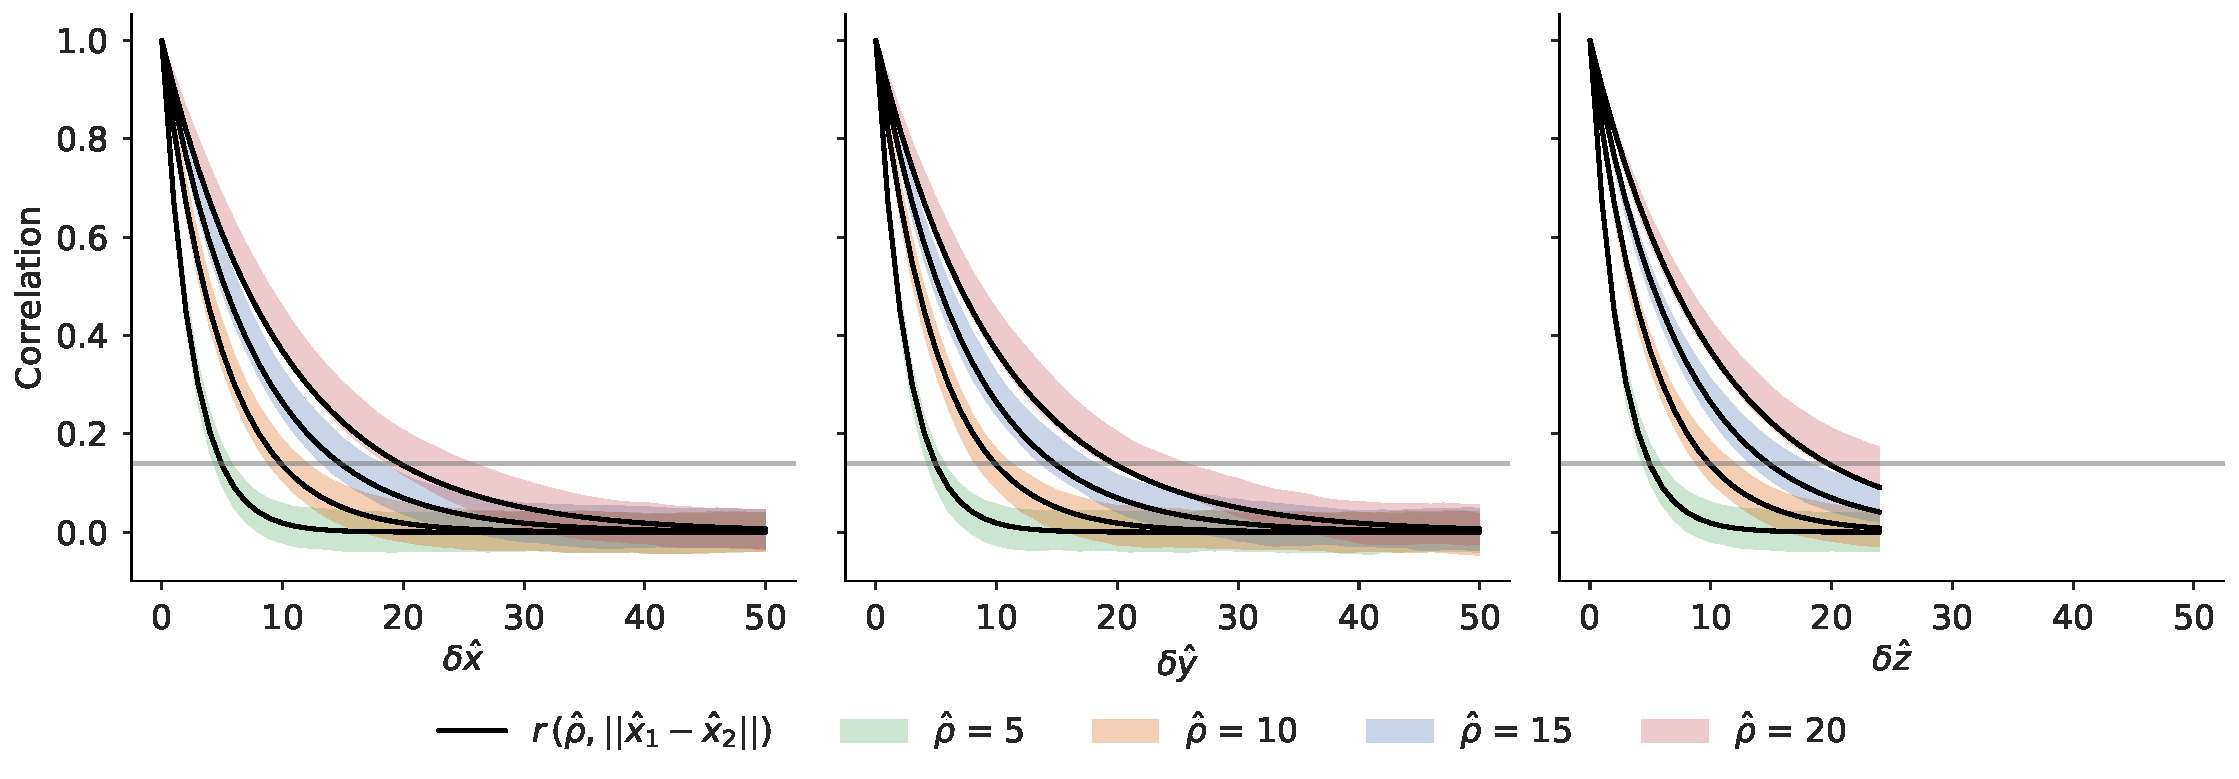
\includegraphics[width=\textwidth]{../figures/matern_llc90_correlation-k25-iy165-ix90-1000samples-4curves.pdf}
    \caption{Correlation coefficient from a subset of the LLC90 in the Pacific
        Ocean, with computations carried out across "inner"
        (158, 118)$^\circ$W,
        (62, 2)$^\circ$S and
        with an "outer" (allowing neighboring interactions spanning out to)
        (178, 98)$^\circ$W,
        (76$^\circ$S, 29$^\circ$N).
        distances computed in each dimension from 1000 samples. The coefficient is
        computed from the random samples used to estimate
        $\hat{\sigma}$ and $X$. Each color denotes correlations computed for a
        different value of $\rangeh$, and the spread is determined by one standard
        deviation around the domain averaged correlation coefficent.
        The black curve denotes the predicted isotropic correlation predicted by
        equation \eqref{eq:matern_correlation_iso} with the appropriate value for
        $\rangeh$.}
    \label{fig:llc90_correlations}
\end{figure}

\subsection{Sample Correlation Maps}
\label{ssec:llc90_correlation_maps}

Maps of the sample correlation field are computed at two locations on the LLC
grid, are shown in
\cref{fig:llc90_correlation_maps}.
For these calculations we use a relatively large correlation length scale
defined by $\rangeh=20$ for illustrative purposes.
First, we compare panels (a) and (b) of \cref{fig:llc90_correlation_maps}, which
show the sample correlation computed at X and Y, respectively.
In panel (a), the correlation structure is anisotropic such that the field is
somewhat ellipsoidal, with relatively correlation length scales that are
relatively longer zonally than meridionally.
On the other hand, the correlation structure shown in panel (b) is closer to
being isotropic, qualitatively speaking, since the field is relatively circular
except where it intersects with the coast.

In this example we obtain longer correlation length scales at the equator
because the LLC grid is defined with smaller meridional grid spacing here in
order to resolve tropical, zonal currents;
see \cref{fig:llc90_correlation_maps}(c) for a comparison of $\Delta x $ and
$\Delta y$ near the equator.
To clarify why this corresponds to the correlation structure we obtain,
consider the normalization of the Laplacian discussed in
\cref{ssec:scaling_laplacian}, and the interpretation of $\rangeh$ described
in \cref{ssec:llc90_correlations}.
Since the meridional grid refines near the equator, the number of grid cells at
which correlation drops to 0.14 covers a shorter distance meridionally compared
to the zonal direction.

\begin{figure}
    \centering
    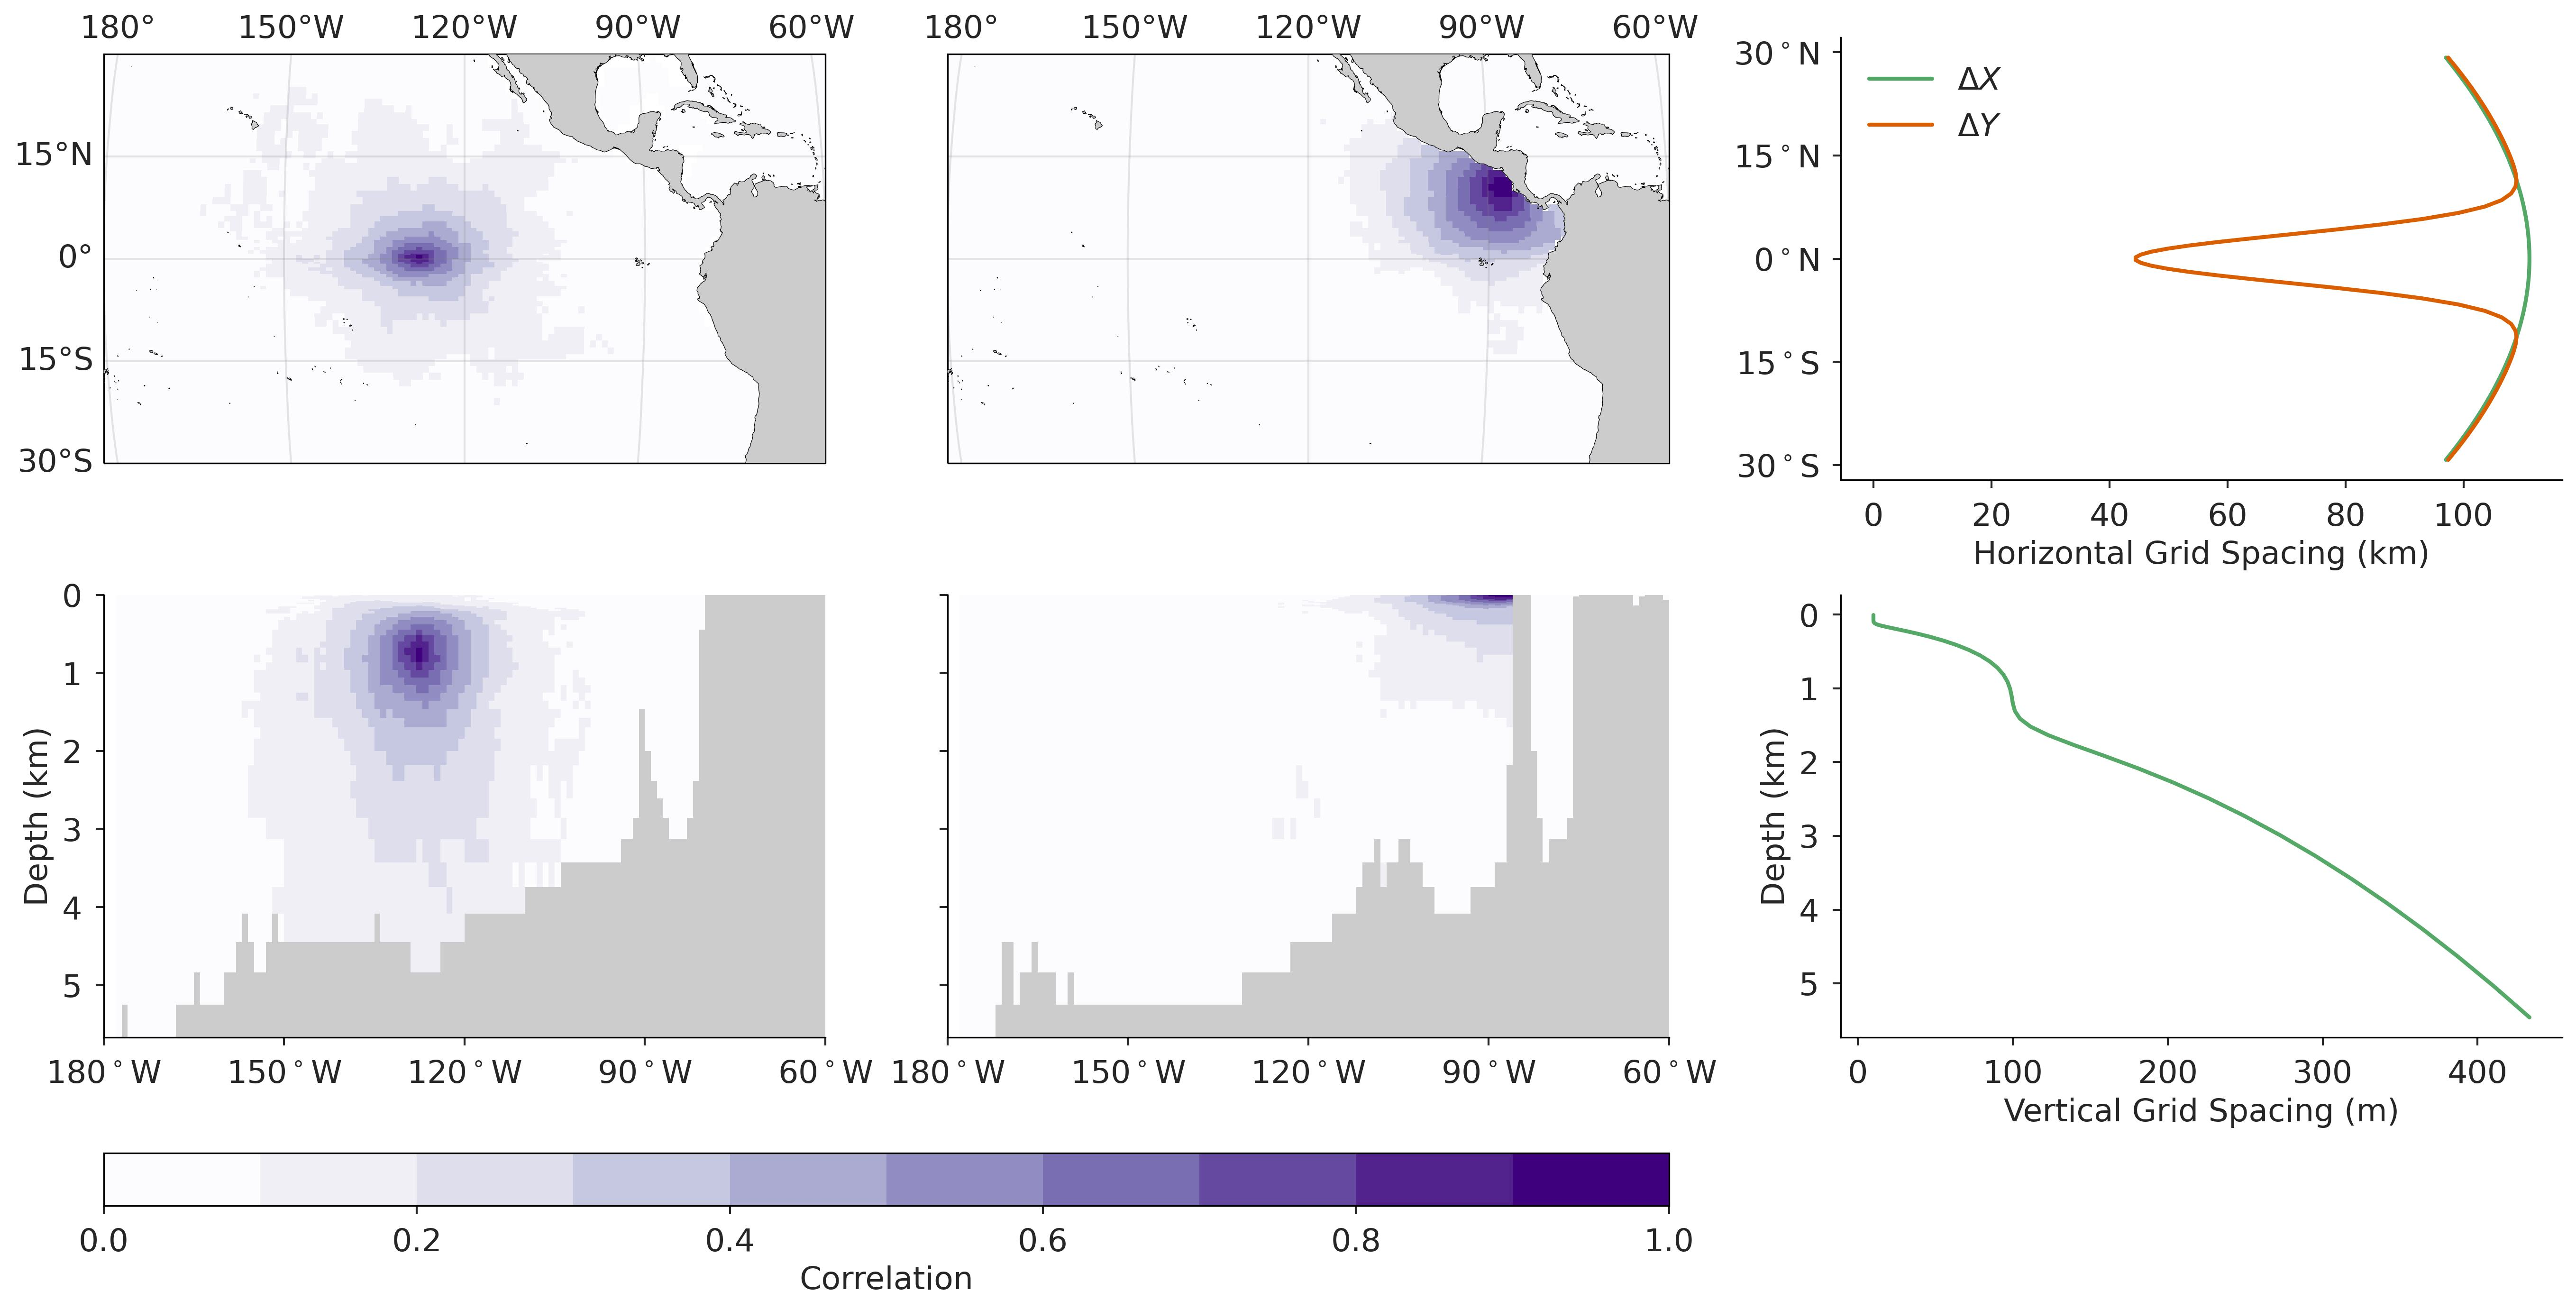
\includegraphics[width=\textwidth]{../figures/huge_correlation_map.jpg}
    \caption{Two sample correlation fields and a depiction of the computational
        grid.
        (a \& b) Sample correlation field in the latitude-longitude plane at
        ( 0.2$^\circ$N, 127.5$^\circ$W, 722~m depth) and
        (10.5$^\circ$N,  87.5$^\circ$W,   5~m depth), respectively.
        (c \& d) The same sample correlation fields as above, shown in the
        depth-longitude plane.
        (e \& f) The local horizontal and vertical grid spacing, respectively.
        The sample correlation fields are computed from 1,000 random samples,
        with $\rangeh = 20$ \red{and $M=1$}.
    }
    \label{fig:llc90_correlation_maps}
\end{figure}

Panels (d) and (e) of \cref{fig:llc90_correlation_maps} show the extent of the
sample correlation fields from (a) and (b) in depth-longitude space,
computed at X and Y depths, respectively.
In panel (d) the correlation remains greater than 0.1 until roughly 3.5-km
depth, whereas the correlation structure in panel (e) is much more confined to
the surface.
Once again, the difference in behavior is due to the fact that the vertical grid
spacing is smaller toward the surface than it is below 1000-m in order to
resolve the ocean mixed layer and surface processes, see
\cref{fig:llc90_correlation_maps}(f).

\subsection{The Normalization Factor}
\label{ssec:llc90_boundary_effects}

The normalization factor for various length scales is shown in \red{FIGXX}.
\red{The colorbar in each figure is normalized such that lightly colored regions
are closer to the} variance expected for an isotropic, stationary Mat\'ern
field \red{REF EQN}.
The largest departure from the analytically derived variance near the
boundaries, \red{similar to wc01}.
However, considering the spatial structure shown in
\cref{fig:llc90_correlation_maps}, using an empirically derived normalization
factor seems satisfactory in removing the boundary effects in order to arrive at
an expected correlation structure.
Other methods to analytically remove boundary effects, for example considered by
\red{CITE}, could be explored in future work.

\subsection{Numerical Considerations}
\label{ssec:tolerance}

One consequence of defining a Mat\'ern field through the sollution involving the
inverse of an elliptic operator is that we must solve a poisson problem.
This solution is obtained most often obtained via an iterative algorith (e.g.\
\cref{sec:block_sor}) which is
terminated after achieving an approximate error that is less than some specified
tolerance.
Within this framework, one can always set a tolerance based on the numerical precision being used
(e.g.\ $10^{-15}$ in double precision as is used here), and remain confident
that the solver has converged.
However, we show here that solving to double precision is often overly ambitious.

To be specific, \cref{fig:error_and_iters}(a) shows the relative error in the
approximation that correlation is equal to 0.14 when $\rangeh = \delta\hat{x}$
for $\rangeh = \{5, 10, 15, 20\}$ (i.e.\ corresponding to the curves in
\cref{fig:llc90_correlations}).
The error in the approximation is shown for a range of poisson solve tolerances,
where $10^{-15}$ is the smallest considerable tolerance for double precision.
Clearly, the error approximation levels off after decreasing the tolerance to
around $10^{-3}$, indicating that the desired statistics of the correlation
model are obtained even with a relatively imprecise solve.

The motivation for using a high tolerance is indicated by
\cref{fig:error_and_iters}(b), which shows how the number of iterations required
to converge increases with the specified tolerance.
Specifically, solving to a tolerance of $10^{-15}$ requires a factor of 6-13
more iterations than are required with a tolerance of $10^{-3}$.
Of course, the specific computational savings obtained will depend on the
iterative method that is being used, but we provide this as a concrete example
to highlight that an inexact solve is both valid and advantageous.

\begin{figure}
    \centering
    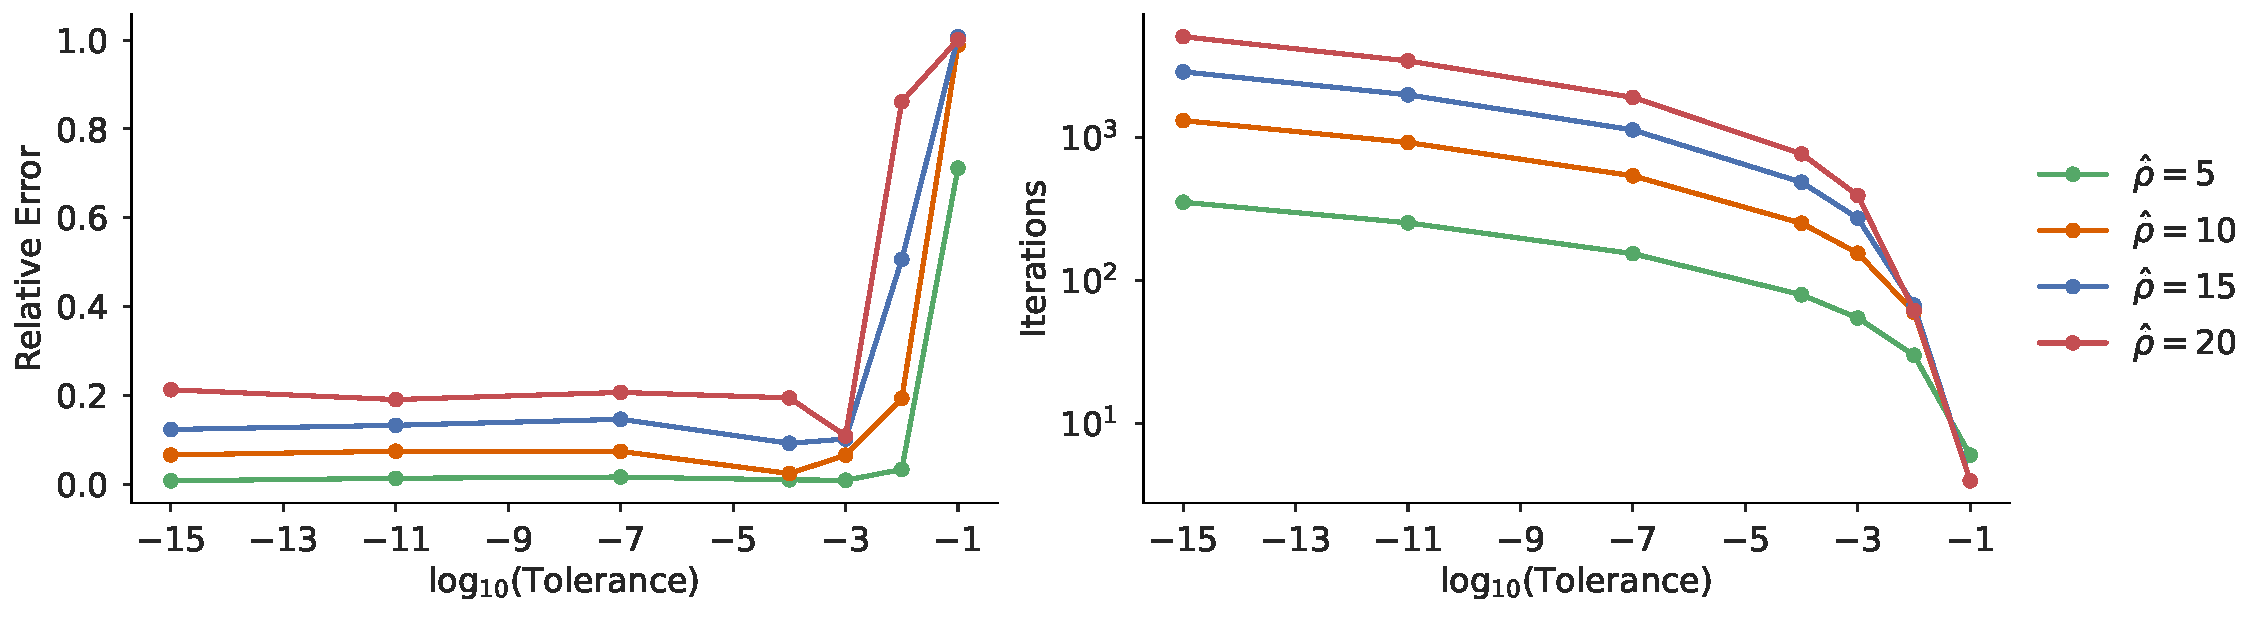
\includegraphics[width=\textwidth]{../figures/matern_llc90_error_and_iters.pdf}
    \caption{(a) The relative error in the approximation that correlation equals
        0.14 when $\rangeh=\delta\hat{x}$, as a function of the tolerance used
        for the iterative block-SOR method described in \cref{sec:block_sor}.
        Each curve is computed as the error between the theoretical (black)
        curve and the average of each colored curve shown in \cref{fig:llc90_correlations}.
        (b) The number of iterations required for the block-SOR method to
        converge to the specified tolerance.
    }
    \label{fig:error_and_iters}
\end{figure}
